\documentclass[UTF8]{ctexart}
\usepackage{graphicx}
\usepackage{float}
\usepackage{geometry}
\usepackage{fancyhdr}
\usepackage{lastpage}
\usepackage{subfigure}
\usepackage{booktabs}
\geometry{left=2.54cm,right=2.54cm,top=3.18cm,bottom=3.18cm}%页边距
\pagestyle{fancy}
\lhead{\includegraphics[scale=1]{sjtu-logo-red.pdf}}  
\rhead{Intel与AMD处理器发展历程报告} 
\cfoot{第 \thepage\ 页\ 共 \pageref{LastPage} 页} 


\begin{document}

\begin{titlepage}
    \begin{center}
        \includegraphics[width=0.8\textwidth]{sjtu-name-blue.pdf}\\[1cm]
        \textsc{\Huge \bfseries 课程报告}\\[1.5cm]
        \includegraphics[width=0.3\textwidth]{sjtu-badge-blue.pdf}\\[0.5cm]

        \Huge \bfseries{Intel与AMD处理器发展历程报告}\\[1cm]
        \Large \bfseries{518021910971 裴奕博}
    \end{center}
\end{titlepage}

\tableofcontents
\newpage
\section{CPU发展概述}
1947年12月,由美国贝尔实验室的肖克利、巴丁和布拉顿组成的研究小组,发明了晶体管。这种新的材料工艺相比之前的真空电子管,体积小巧、无需预热、耗能极低,很快取代了电子管成为了新一代电子电路的首选。在随后的几十年间,伴随着集成电路的发明,由这种材料制成的电子电路规模越来越大。从小规模、中规模集成电路到大规模、超大规模集成电路。
\begin{figure}[H]
    \begin{center}
        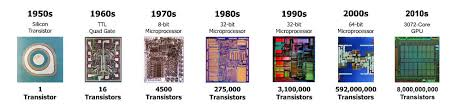
\includegraphics[width=0.8\textwidth]{figure/ICdev.jpg}
        \caption{集成电路的发展}
    \end{center}
\end{figure}

随着人类对计算机计算能力和便携性的要求不断提升,人们提出了“微型计算机”的概念,要实现这一点,首当其冲的就是将计算机的中央处理单元小型化。1971年,Intel公司制造出了第一个商用微处理器即4004,也宣告了第四代计算机时代的来临。从1971年至今的近50年间,随着个人计算机(PC)的成熟、发展和普及,作为计算机核心的CPU也得以迅猛发展。两家“本是同根生”的半导体公司,Intel和AMD,在这几十年间共同促成了CPU技术的不断提升,时至今日也是市面上处理器的最主流选择。本报告即梳理了从1971年至今,两家公司系列处理器的发展历程。
\newpage
\section{Intel系列处理器发展历程}
1968年创立的Intel,是全球目前收入和市值最高的半导体公司,总部位于美国加州圣克拉拉。1971年,Intel的工程师发明了世界上第一款CPU4004。在之后的几十年间,集成电路的制造工艺和架构在不断进化,Intel却始终在大部分事件都在处理器市场中占据主导地位。本章将详细讲述Intel系列处理器的发展历程。

\begin{figure}[H]
    \begin{center}
        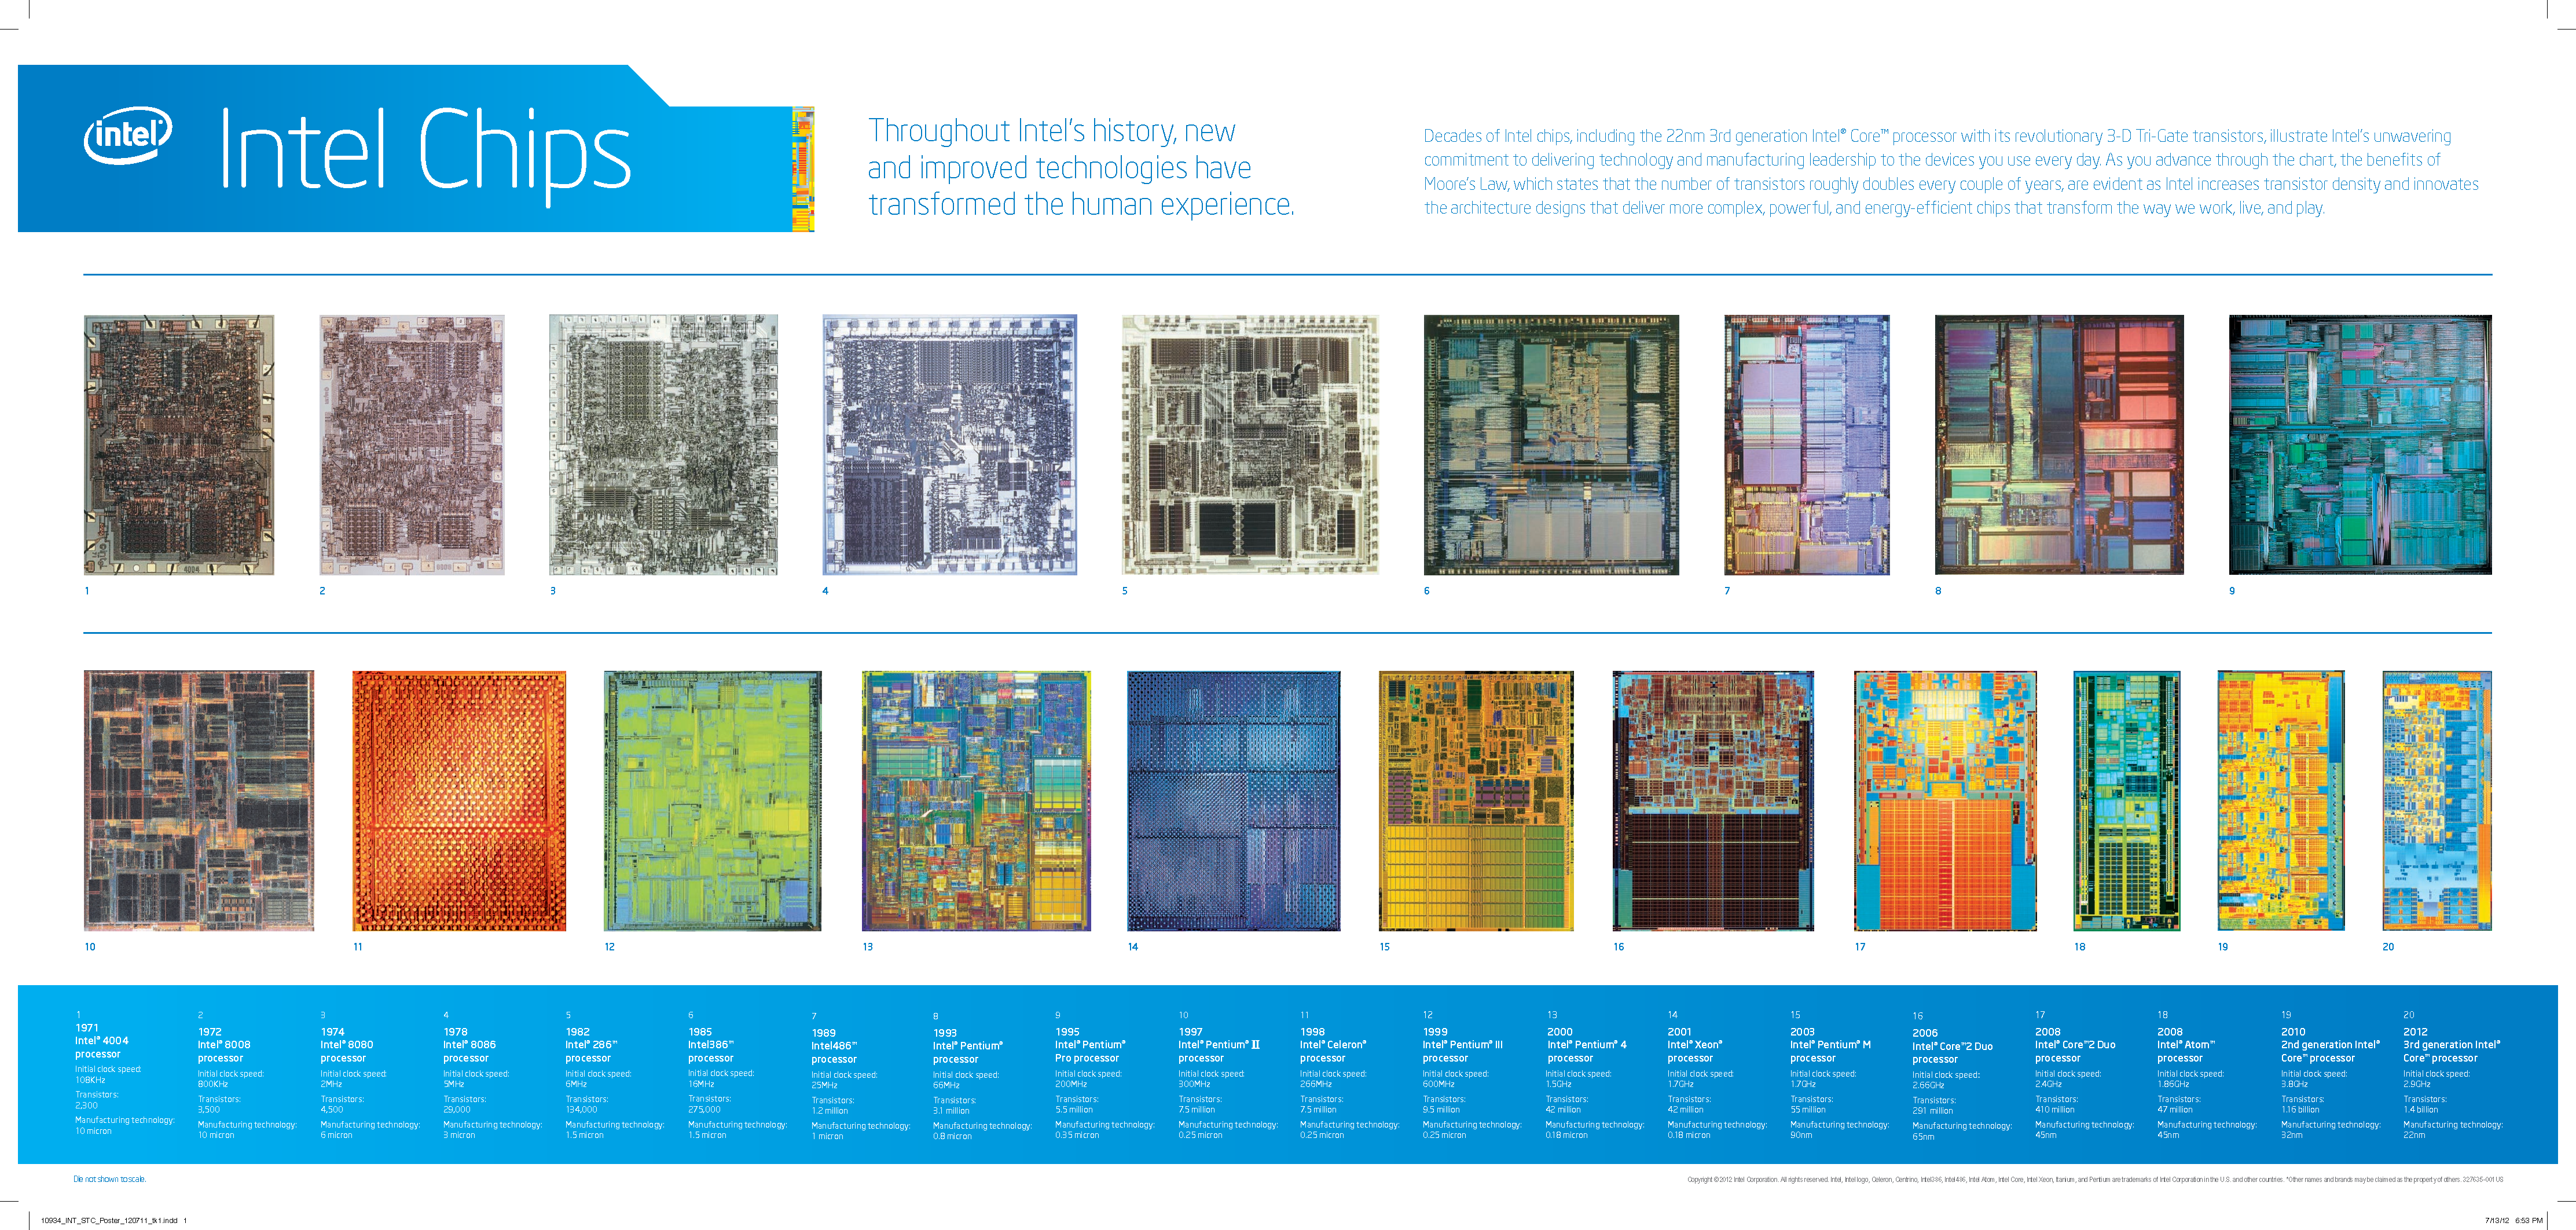
\includegraphics[width=\textwidth]{figure/inteldev.jpg}
        \caption{Intel系列处理器的发展}
    \end{center}
\end{figure}

\subsection{1968-1978 Intel公司的创立与4004处理器的诞生}
\subsubsection{Intel的创立}
1955年,晶体管的发明者威廉·肖克利离开贝尔实验室,创建了肖克利半导体实验室,并且吸引了一大批有才华的年轻科学家加入。但很快,由于内部原因,其中8名科学家联合辞职创办了仙童半导体公司,其中就包括摩尔定律的提出者戈登·摩尔(Gordon Moore)和集成电路的联合发明人罗伯特·诺伊斯(Robert Noyce)。1968年,两人从仙童半导体公司辞职,在7月16日共同创办Intel公司。其名称来源于集成电路(Integrated Electronics)的首字母缩写。
\begin{figure}[H]
    \begin{center}
        
\includegraphics[width=0.2\textwidth]{figure/intel.png}
        \caption{Intel公司现在的logo}
    \end{center}
\end{figure}
起初,Intel的业务主要来自半导体存储器市场,主攻DARM和SARM,在整个20世纪70年代,CPU都不是Intel最主要业务。1971年11月15日,Intel的工程师霍夫(Marcian Hoff)发明了世界上第一块大规模集成电路,也是第一颗微处理器Intel 4004。恐怕那时Intel公司自己也未曾想到,这一天将被永远载入史册,这一“无心之举”也成为了Intel在今后几十年绝大部分的收入来源。

\subsubsection{Intel 4004}
4004处理器起初只是用于在日本Busicom公司生产的计算器中替换一些应用导向集成电路。它只有4位,45条指令,最高主频也仅有740kHz,甚至比不上ENIAC。但由于它集成化程度高,体积小,为个人计算机的发展铺平了道路,具有重要的里程碑意义。
\begin{figure}[H]
    \begin{center}
        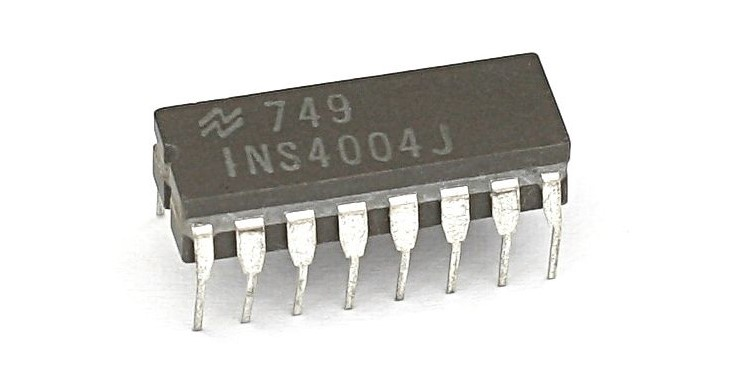
\includegraphics[width=0.4\textwidth]{figure/4004.jpg}
        \caption{Intel 4004}
    \end{center}
\end{figure}

\subsubsection{Intel 8008/8080}
在接下来的几年中,Intel又推出了8位的8008(1972)和8080(1974)处理器。在研发8008的过程中,Intel还获得了由德州的Datapoint公司开发的指令集,正是这套指令集,奠定了今天x86系列指令集的基础。与此同时,微处理器的优势也逐渐被人们所认同。尤其是8080处理器获得了空前的成功。该处理器主频为2MHz,性能是8008的十倍。作为人类历史上的第一台个人计算机Altair也使用了8080处理器作为核心。
\begin{figure}[H]
    \centering
    \subfigure[Intel 8008]{
        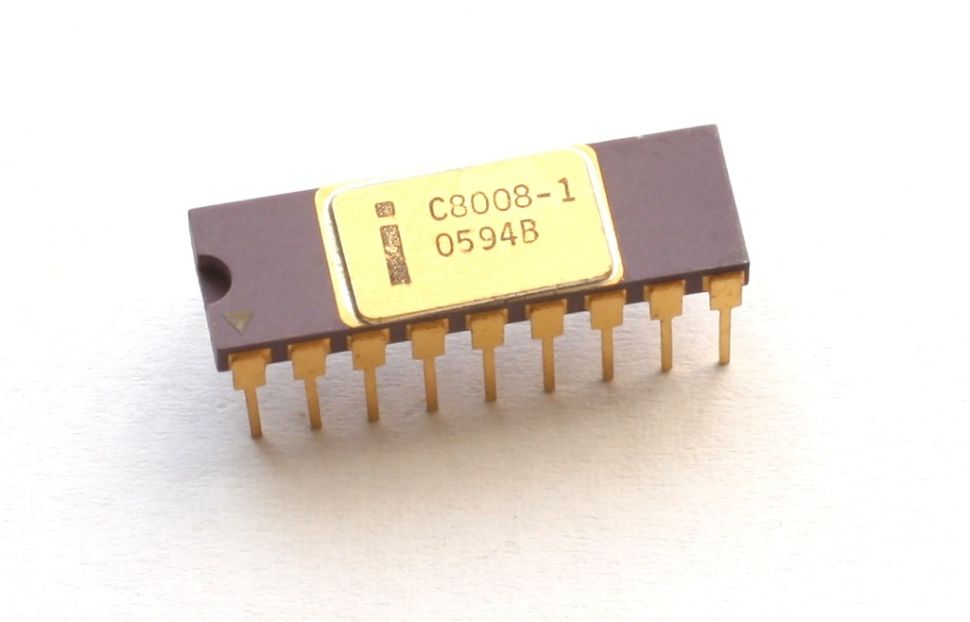
\includegraphics[width=0.4\textwidth]{figure/8008.jpg}
    }
    \subfigure[Intel 8080]{
        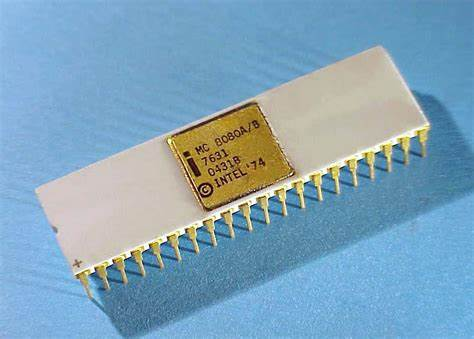
\includegraphics[width=0.3\textwidth]{figure/8080.jpg}
    }
    \caption{Intel 8008/8080}
\end{figure}

\subsection{1978-1993 x86系列处理器与x86指令集的开端}
这一阶段,Intel以8086处理器为开端,开创了x86指令集架构,这一架构也对未来的处理器发展有着深远影响。
\subsubsection{Intel 8086/8088}
1978年,Intel推出了8086处理器。它有16位的数据总线,可一次读取1MB内存,是Intel推出的首个16位处理器。与此同时,Intel还在其上使用了x86指令集。子从那时起,几乎所有的Intel和AMD处理器的指令集都是基于该指令集。从此,x86也成为了个人计算机的标准平台,也是历来最成功的CPU架构之一。

几乎与此同时,Intel也推出了8088处理器,将地址总线提升至20bit。两款处理器都采用了相同的16位x86架构。
\begin{figure}[H]
    \begin{center}
        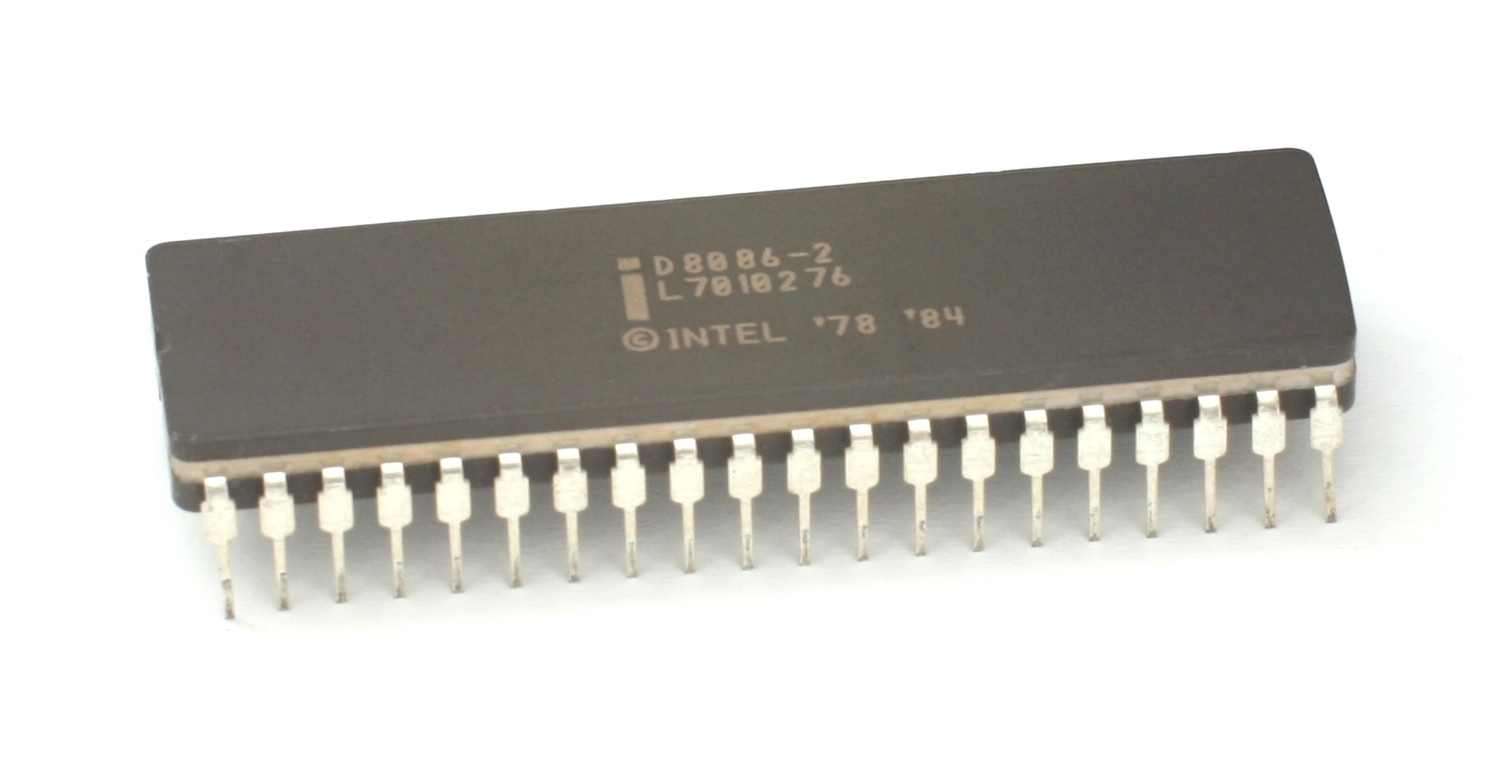
\includegraphics[width=0.3\textwidth]{figure/8086.jpg}
        \caption{Intel 8086}
    \end{center}
\end{figure}

\subsubsection{Intel 80x86系列}
随着PC市场需求的一步步扩大,CPU业务逐渐成为了Intel的主业。从1980年起,Intel接连推出了一系列基于x86架构的处理器,包括80186(1980)、80188(1980)、80286(1982)、80386(1985)和80486(1989)。
\begin{figure}[H]
    \centering
    \subfigure[Intel 80186]{
        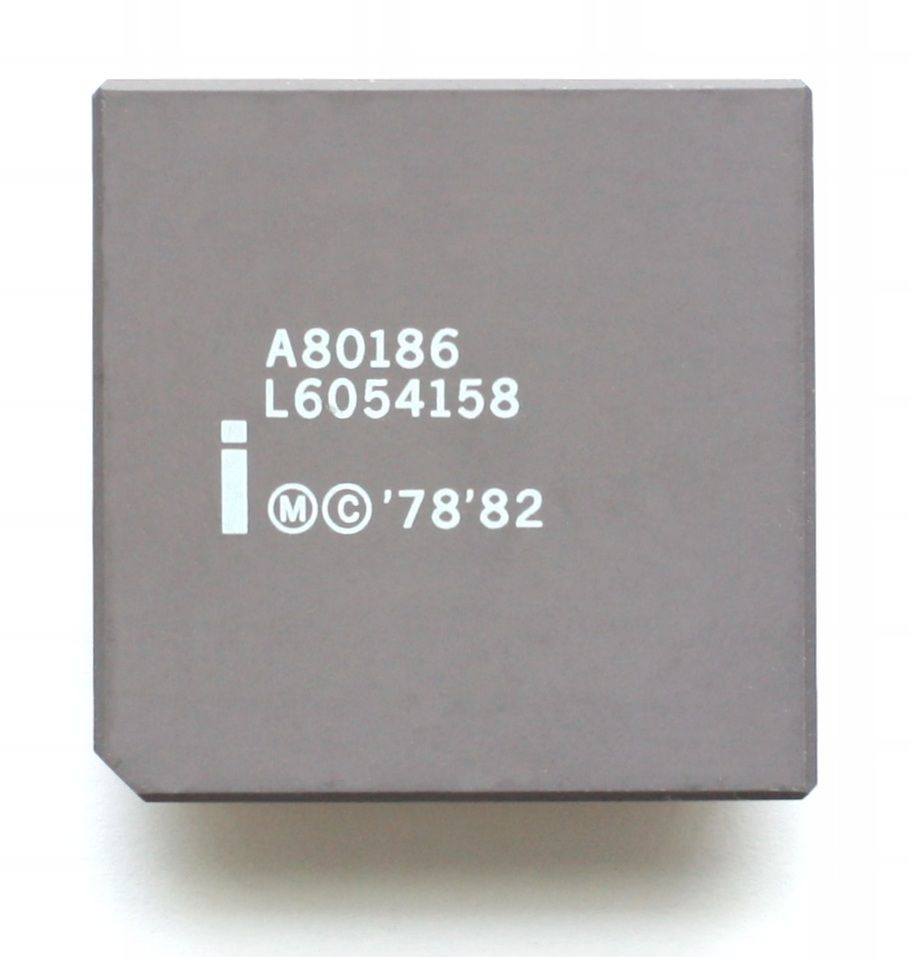
\includegraphics[width=0.25\textwidth]{figure/80186.jpg}
    }
    \subfigure[Intel 80486]{
        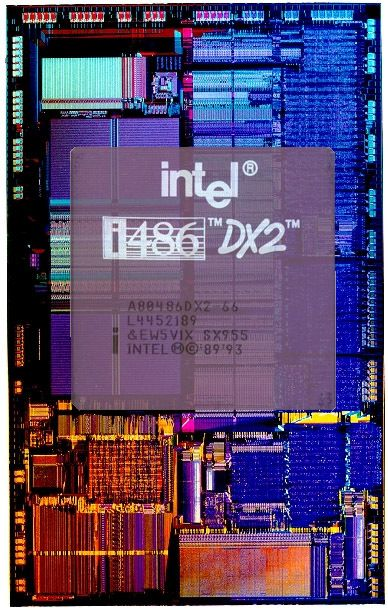
\includegraphics[width=0.18\textwidth]{figure/80486.jpg}
    }
    \caption{Intel 80186和80486}
\end{figure}
其中,80188和80186几乎同时推出,80188削减了一半的外部数据总线以降低成本。80286是Intel第一款完全兼容前代CPU的处理器。

从1985年的80386开始,Intel系列处理器进入32位时代,32位的x86架构也称为IA-32。80386集成了27万多只晶体管,规模超过了了初代CPU 4004的100倍,同时也是第一款具有多任务功能的处理器,这也为操作系统的发展有重要影响。

1989年,Intel发布了最后一款用数字命名的处理器——Intel 80486。在这一代CPU上,Intel首次将FPU(浮点计算单元)集成在CPU之内。此外,8KB的L1缓存第一次出现在了x86 CPU上。


\subsection{1993-2006 奔腾(Pentium)时代}
经过一系列80x86处理器,Intel已经从一家主攻存储芯片的公司,转为CPU领域的霸主。1993年,Intel发布了以子商标奔腾(Pentium)命名的处理器,正式宣告处理器进入奔腾时代。
\subsubsection{Pentium与Pentium MMX}
1993年,采用P5架构的Pentium处理器发布,而没有遵循80x86号码系统。这是一个划时代的事件。在接下来的十几年间,奔腾几乎成为了家喻户晓的名字,时至今日仍在使用。初代Pentium系列将CPU的工作电压降至3.3V,增强了浮点数的运算,新使用的P5架构使得它在所有方面都比80486快。1994年,Pentium处理器被发现在浮点数的计算上出现了瑕疵,Intel不得不召回大批的Pentium处理器。

然而这一事件并未影响Intel在CPU领域的高歌猛进。1996年,主攻服务器方向,采用P6架构的Pentium Pro推出。1997年1月,Pentium MMX推出。它扩展了L1缓存至16KB,也扩展了新的MMX指令集,使得其对多媒体数据的处理更为强大,也因此红极一时。此外,MMX系列的处理器还拥有较强的超频能力,还能通过提高其核心电压来获得更好的性能。1997年,同样采用P6架构的Pentium \uppercase\expandafter{\romannumeral2}发布,L1缓存已经增加到16KB数据缓存+16KB指令缓存共32KB。
\begin{figure}[H]
    \centering
    \subfigure[Pentium MMX]{
        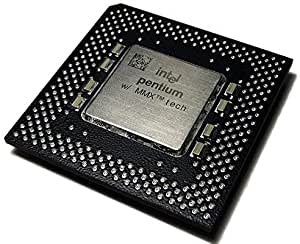
\includegraphics[width=0.25\textwidth]{figure/pentium.jpg}
    }
    \subfigure[Pentium Pro]{
        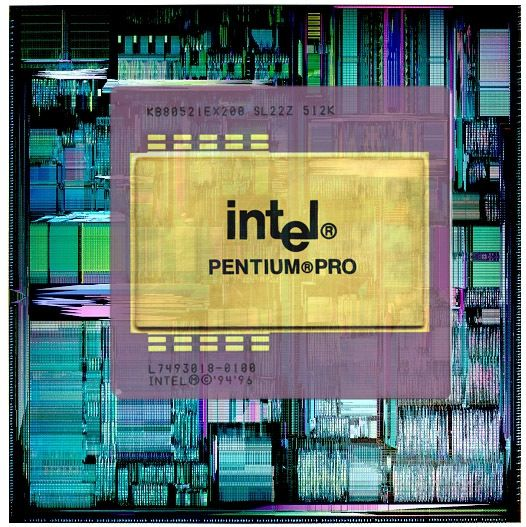
\includegraphics[width=0.2\textwidth]{figure/pentium_pro.jpg}
    }
    \caption{Pentium和Pentium Pro}
\end{figure}

\subsubsection{赛扬(Celeron)和至强(Xeon)}
1998年,随着AMD大举入侵低价处理器市场,而同期的Pentium \uppercase\expandafter{\romannumeral2}价格昂贵。为了兼顾低端市场,Intel将Pentium \uppercase\expandafter{\romannumeral2}中的两颗L2缓存取消,推出了初代Celeron处理器,从此诞生了“赛扬”这一新的产品线。

同时,为区分服务器市场与PC市场,英特尔还推出了Pentium \uppercase\expandafter{\romannumeral2} Xeon作为Pentium Pro的升级产品,从此诞生了Xeon处理器。直到2001年,Intel将Xeon系列前面的Pentium取消,从此独立出面向中高端服务器市场的Xeon系列。

时至今日,Celeron和Xeon系列仍然是Intel CPU中最低端和高端的代表。而它们都脱胎于当年的Pentium系列。
\begin{figure}[H]
    \centering
    \subfigure[Celeron]{
        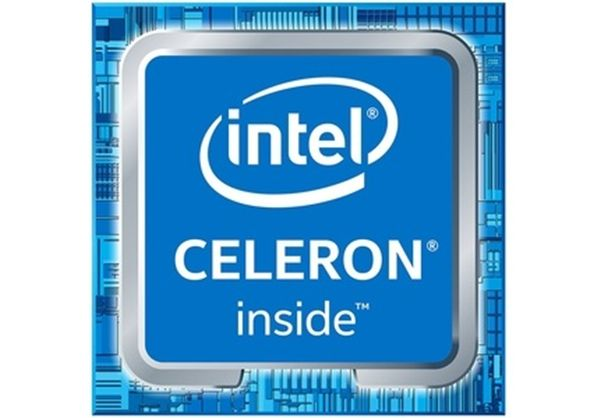
\includegraphics[width=0.22\textwidth]{figure/celeron.jpg}
    }
    \subfigure[Xeon]{
        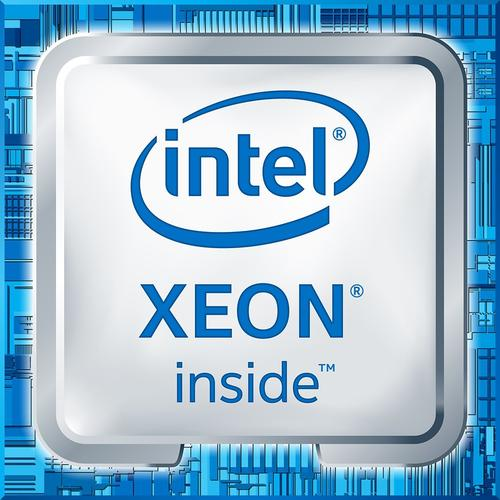
\includegraphics[width=0.15\textwidth]{figure/xeon.jpg}
    }
    \caption{Celeron和Xeon系列}
\end{figure}

\subsubsection{Pentium系列的后续产品}
世纪之交,Pentium系列产品的更新迭代还在继续。Intel相继推出了Pentium \uppercase\expandafter{\romannumeral3}(1999)、Pentium 4(2000)、Pentium M(2004)和Pentium D处理器。

其中,1999年推出的Pentium \uppercase\expandafter{\romannumeral3}处理器的主频首次突破1GHz。2002年,Intel在Pentium 4上首次运用了超线程技术。2005年,带有两个处理器内核的Pentium D推出,开启了CPU多内核的时代。以上三点是Pentium系列在这几年中主要的创新点。

然而在这一时期,从Pentium 4开始使用的P4架构“Netburst”出现了功耗和热量问题,在很长一段时间内,Intel无法将Netburst架构的处理器主频升至2GHz以上。随后,在此基础上改进的“Prescott”架构(被用于Pentium D)同样也出现了类似的问题。在一段短暂的时间中,Intel的在CPU领域的统治被AMD所打破。这也迫使Intel放弃Netburst架构,转而支持基于P6的Pentium M设计,这也促成了Intel新一代产品酷睿(Core)的诞生。

\subsection{2006-至今 酷睿(Core)的又一次辉煌}
随着AMD的步步紧逼,Intel不得不调整自己的策略。从2005年开始,Intel制定了一套“钟摆计划”(Tick-Tock),并在2006年推出了新一代酷睿(Core)产品,重新逆转了与AMD的竞争局面。时至今日,Core系列产品仍是广大消费者选择CPU的不二之选。
\subsubsection{Core 2 Duo:初代Core}
从2004到2006,Intel陷入了一段低迷时期。AMD凭借其K8系列,以“真双核”和较好的能效比赚足了世人的眼球。为了从AMD手中重新夺回CPU市场的主导地位,Intel启动了Tick-Tock计划,即用时钟的声响(Tick,Tock为拟声词)代表芯片制程和处理器微架构的更新。2005年,Core一代产品发布,标志这Core系列处理器的诞生。此时的Core,架构源自Pentium M,而新架构的开山之作,即是2006年7月发布的Core 2 Duo。
\begin{figure}[H]
    \centering
    \subfigure[]{
        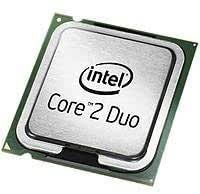
\includegraphics[width=0.2\textwidth]{figure/core2duo.jpg}
    }
    \subfigure[]{
        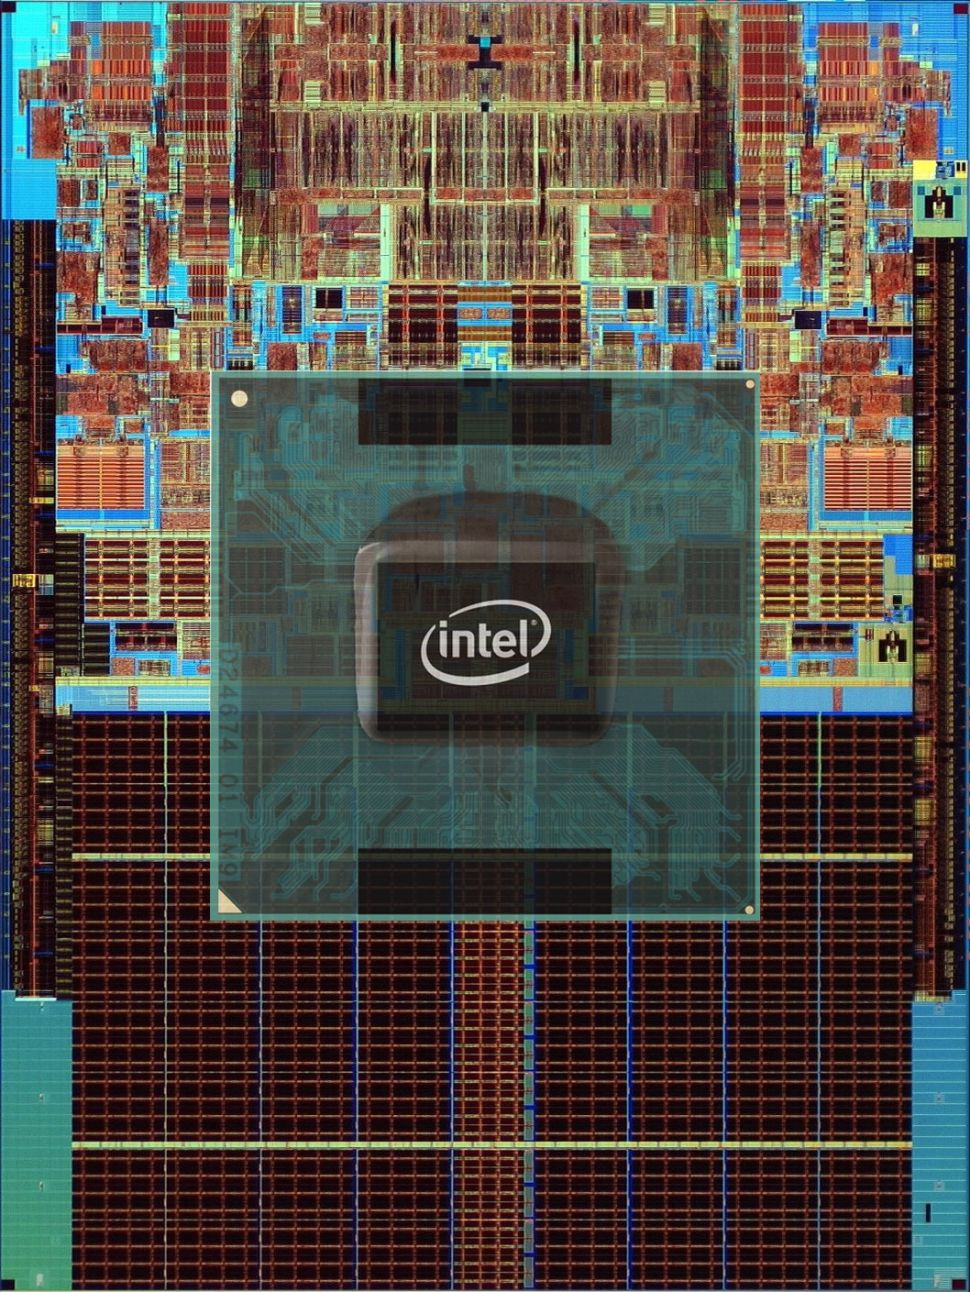
\includegraphics[width=0.15\textwidth]{figure/core2duoin.jpg}
    }
    \caption{Core 2 Duo}
\end{figure}

Core 2 Duo采用了65nm制程工艺,Intel声称它对比上一代产品有40\%的性能提升,同时减少40\%的功耗,各项数据均大幅领先当时AMD的Athlon 64X2。从此,Intel再次夺回了CPU的主导权。

究其原因,Core 2 Duo抛弃了此前出现各种问题的Netburst架构,转而对Pentium M的微架构进行改进,定名Core架构。Core 2 Duo为双核心64位处理器,将双核共享的L2缓存提升至4MB,晶体管总数达到近3亿个,此外还加入了对EM64T与SSE4指令集的支持,使其拥有更强大的寻址空间。Core微架构的改进,实现了能效比的大幅提升。

此后,由于Core架构的巨大成功,Intel将其也运用到了Celeron、Pentium乃至Xeon产品线中。

\subsubsection{i系列处理器:更清晰的产品定位}
随着Core 2 Duo的发布,Intel的优势再一次被确立,在随后的几年中,Tick-Tock战略稳步实施。2008年,Intel推出的新的Nehalem微架构,引入了新的命名方案。共有三个变体,Core i3,Core i5和Core i7。2008年11月17日,Intel推出了四核的Core i7处理器。2009年9月8日,第一款Core i5发布。2010年1月7日,首款Core i3发布。i3,i5和i7分别针对入门级消费者,普通消费者和高端消费者,但不再以核心数等技术指标命名。
\begin{figure}[H]
    \begin{center}
        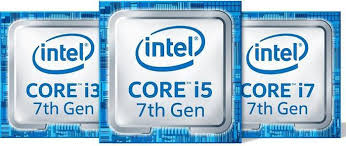
\includegraphics[width=0.35\textwidth]{figure/core1.jpg}
        \caption{Intel Core i系列}
    \end{center}
\end{figure}

在此后的几年中,Intel的i系列处理器陆续推出了一代(Nehalem微架构,45nm,2008),二代(Sandy Bridge微架构,32nm,2011),三代(Ivy Bridge微架构,22nm,2012),四代(Haxwell微架构,22nm,2013)处理器。随着制程和微架构的提升,Core处理器的性能也稳步提升。其中有几个比较有突破性的进展:在Core一代中的部分处理器首次集成了图形处理单元(GPU),Core i7在2010年首次发布了六核处理器,Core二代产品首次支持高性能DDR3内存等。经过几年的产品迭代改进,Intel Core系列在消费级CPU中已经形成了一家独大的局面。

\subsubsection{14nm的爆发}
2015年,CPU制程已经提升至14nm,intel也发布了基于14nm制程的Broadwell微架构的第五代Core处理器。这一代产品的高端型号甚至出现了8核甚至10核的夸张表现。此后发布的第六代(Skylake,2015),第七代(Kaby Lake,2016),第八代(Coffee Lake,2017/Whiskey Lake,2018),第九代(Coffee Lake,2018)Core处理器同样基于14nm制程。

在此期间,Intel两次提升了台式机处理器中的CPU核心数和线程数。在2017年5月,还发布了全新的Core i9系列,作为Core系列的旗舰产品。
\begin{figure}[H]
    \centering
    \subfigure[Intel Core i9]{
        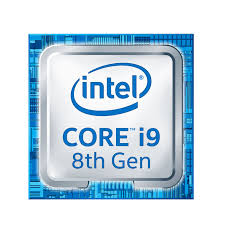
\includegraphics[width=0.17\textwidth]{figure/corei9.jpg}
    }
    \subfigure[Intel Core 10th gen]{
        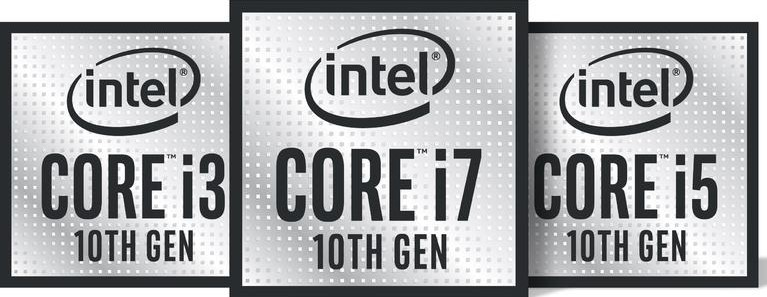
\includegraphics[width=0.4\textwidth]{figure/core10.jpg}
    }
\end{figure}


2019年,Core十代处理器发布,包括部分基于10nm制程,Comet Lake架构的处理器。Intel的处理器制程第一次突破了14nm。2020年9月3日,Intel发布了最新一代的Core 11代低功耗处理器,代号Tiger Lake。
\begin{table}[H]
    \centering
    \caption{Intel核心数与线程数的发展}
    \begin{tabular}{cccc}
        \toprule
        型号    & 第七代 & 第八代 & 第九代 \\
        \midrule
        Core i3 & 2C/4T  & 4C/4T  & 4C/4T  \\
        Core i5 & 4C/4T  & 6C/6T  & 6C/6T  \\
        Core i7 & 4C/8T  & 6C/12T & 8C/8T  \\
        Core i9 & /      & /      & 8C/16T \\
        \bottomrule
    \end{tabular}
\end{table}
\newpage



\section{AMD系列处理器发展历程}
与从一诞生就开始引领整个CPU行业发展的Intel有所不同,比Intel只晚成立1年的Advanced Micro Devices(AMD)公司,起初只是Intel CPU的代工厂。然而AMD通过自身的发展运营,逐步在Intel主导的CPU市场中占有一席之地,始终与Intel处于高强度的竞争之中,甚至有一段时间还盖过了Intel的风头。本章接下来就将详细讲述AMD处理器的发展历程。
\begin{figure}[H]
    \begin{center}
        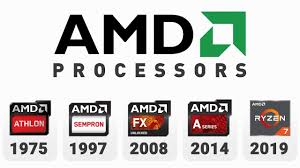
\includegraphics[width=0.6\textwidth]{figure/AMDdev.jpg}
        \caption{AMD处理器的发展历程}
    \end{center}
\end{figure}

\subsection{1969-1991 AMD公司的创立和与Intel的合作}
\subsubsection{AMD的创立}
1969年,杰里·桑德斯(Jerry Sanders)和他的七个同事,一起从仙童半导体公司辞职,创办了AMD公司。杰里·桑德斯本人也从仙童半导体公司的营销总监转身变为了AMD的创始人。因此,两家公司可谓是同源共生。


\subsubsection{早期产品:从仿制开始}
相比Intel创立之初的高声望,AMD创立之初时略显寒酸,甚至一开始只能在创始人的家中办公。为了弥补技术上的落后,AMD从创立之初便确立了自己第二供应商的地位,与Intel的技术导向不同,走物美价廉的路线尽快占领市场。

1974年INTEL推出了8080芯片,一种史上最成功的8位处理器。在那时,8080就是行业的标杆,各国的各大公司纷纷启动仿造,AMD也不例外。1975年,AMD推出了8080的仿造版AM8080,采用了与Intel完全相同的设计。
\begin{figure}[H]
    \begin{center}
        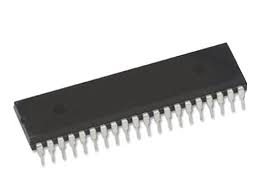
\includegraphics[width=0.3\textwidth]{figure/AM8080.jpg}
        \caption{AMD的第一款处理器AM8080}
    \end{center}
\end{figure}

\subsubsection{AMD与Intel的合作}
1978年,随着Intel 8086处理器的推出,CPU正式进入x86时代,而AMD只能等待Intel的生产授权。然而,转机发生在1981年,IBM创建了PC并想要Intel的x86处理器,但前提是英特尔必须为其专利的x86微处理器提供第二来源的制造商。就这样,在IBM的推动下,AMD与Intel签署了长达十年的合作协议,后来又延长至1995年。协议的结果是:AMD成为英特尔的x86微处理器和相关芯片的第二制造商,英特尔提供了其8086,80186和80286芯片的制造权给AMD。

有了这一合作协议,AMD得以继续仿制Intel的处理器。1982年1月,AMD推出了第二款处理器:仿自Intel 80286的AM286。它们有着相同的架构,然而AMD将其时钟频率由12.5MHz提升到了20MHz,而且以更低廉的价格占据了更多的市场。此时,Intel开始意识到,AMD的地位开始对自己构成了威胁。

\begin{figure}[H]
    \begin{center}
        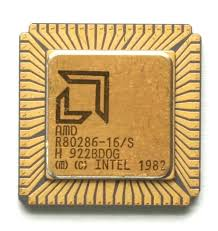
\includegraphics[width=0.2\textwidth]{figure/AM286.jpg}
        \caption{AMD的第二款处理器AM286}
    \end{center}
\end{figure}

\subsection{1991-1999 从AM386到K6:自研CPU的初尝试}

\subsubsection{386的争端}
1985年,Intel推出了80386处理器,感受到威胁的他们单方面撕毁了协议,拒绝给予AMD生产授权,AMD见状只能一纸诉状将Intel告上法庭。在与Intel在法庭周旋的过程中,AMD眼看要错过80386的黄金时期,在另一边开始了自己自研CPU的道路。

时间来到1991年,AMD终于赶在Intel 80486发布前,发布了仿制的AM386处理器。在386处理器上,AMD同样采取了相同的做法:将主频从33MHz上调到了40MHz。

当Intel的80486发布,AMD又仿制了AM486和AMD 5x86处理器,均是由80486提升主频而来。与Intel 80486相同,这两款处理器增加了L1缓存,并将FPU集成到了CPU中。

\subsubsection{K5:AMD的第一款自研处理器}
20世纪90年代,随着与Intel的合作协议到期,AMD只能转而寻求CPU自研。1996年,AMD发布了第一款完全在内部设计的x86处理器。这是一款采用RISC指令集的处理器,解决了传统X86架构因为指令码长度大小不一、管线分配不均匀所造成的性能瓶颈。K5的外部数据总线由原来的32位扩大到64位,L1缓存升级到24KB,并支持主板上的L2缓存,大大提高了数据命中率。
\begin{figure}[H]
    \begin{center}
        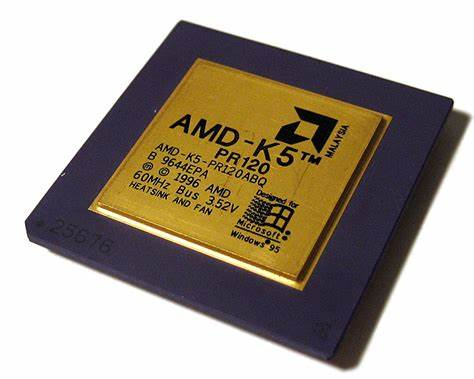
\includegraphics[width=0.3\textwidth]{figure/K5.jpg}
        \caption{AMD的第一款自研处理器K5}
    \end{center}
\end{figure}
然而,正是这样一款技术指标很高的新一代处理器,却遭到了市场的冷遇。其原因是新一代的K5处理器与Intel同时代的Pentium系列处理器并不兼容,这使得厂商需要设计新的主板和接口。对于处理器技术尚未成熟,还只是一个二线厂商的AMD来说,这是市场大忌。直到1996年,AMD才推出了与之兼容的K5处理器,然而为时已晚,Intel已经推出了Pentium Pro处理器,K5仅有的优势已经荡然无存。

\subsubsection{K6:第一款成功的自研处理器}
吸取了之前K5的教训,1997年,AMD在新一代K6架构的处理器上原生支持了Intel的Socket7接口,还兼容了Intel的MMX指令集,提升了对多媒体信息的处理能力。此外,还支持64KB的L1缓存.然而不久,Intel又推出了Pentium \uppercase\expandafter{\romannumeral2}处理器,此时K6还未能动摇Intel的市场。
\begin{figure}[H]
    \begin{center}
        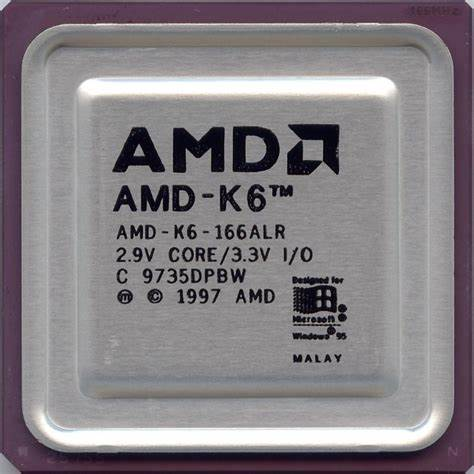
\includegraphics[width=0.2\textwidth]{figure/K6.jpg}
        \caption{AMD K6处理器}
    \end{center}
\end{figure}
然而,AMD却在其中看到了机会:Intel在Pentium \uppercase\expandafter{\romannumeral2}处理器采用了全新的Slot1接口,封杀了其他兼容厂商。但与此同时,AMD抓住了消费者不愿为Pentium \uppercase\expandafter{\romannumeral2}更换新主板的心理,于1998年推出了K6-\uppercase\expandafter{\romannumeral2}处理器。K6-\uppercase\expandafter{\romannumeral2}在性能指标上提升巨大,支持了512KB到2MB的L2缓存,并添加了3DNow指令集,让K6-2可以执行浮点SIMD指令,大大增强了K6-2的浮点运算和3D图形能力。相比Pentium\uppercase\expandafter{\romannumeral2},K6-\uppercase\expandafter{\romannumeral2}以三分之一的价格和超过其三分之二的性能,取得了巨大的成功,此时的AMD,已经可以在CPU市场上与Intel有了一战之力。

1999年,AMD趁热打铁又推出了K6-\uppercase\expandafter{\romannumeral3}处理器。K6-\uppercase\expandafter{\romannumeral3}首次将主板上的L2缓存集成到了CPU中,支持主板上的512KB到2MB的L3缓存,相比K6-\uppercase\expandafter{\romannumeral2}在晶体管数量上提升了超过一倍,达到了2130万个。然而K6-\uppercase\expandafter{\romannumeral3}价格比较昂贵,很快便被后续的Athlon(速龙)处理器替代。


\subsection{1999-2006 Athlon系列:AMD的崛起和辉煌}

\subsubsection{初代Athlon:和Intel分庭抗礼的开始}
由于K6-\uppercase\expandafter{\romannumeral3}价格昂贵,AMD在1999年又推出了新的基于K7架构的处理器,命名为Athlon(速龙)。这一代处理器抛弃了之前的Socket7接口,是AMD第一个具有SMP(对称多处理器)技术的桌面CPU,用户可以由此构建多处理器的系统。此外,初代的Athlon处理器还拥有128KB的L1缓存和512KB的L2缓存。
\begin{figure}[H]
    \begin{center}
        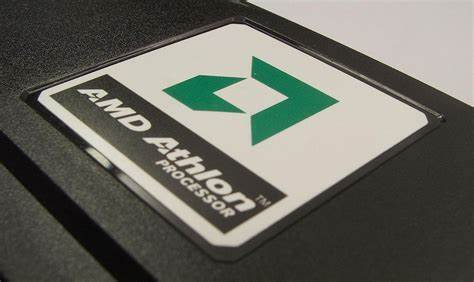
\includegraphics[width=0.3\textwidth]{figure/athlon.jpg}
        \caption{AMD Athlon处理器}
    \end{center}
\end{figure}
和同时期的Pentium \uppercase\expandafter{\romannumeral3}处理器相比,Athlon与其不分伯仲,甚至在浮点数计算和游戏场景中更胜一筹。从此,AMD终于迎头赶上,在同一时期与Intel形成了几乎对等的竞争。
\subsubsection{Athlon系列的发展}
1999年底,AMD又推出了Athlon系列的改进版,由于采用了180nm工艺,CPU得以在更高的主频上运行。2000年3月,AMD抢先发布了世界上第一款1GHz处理器Athlon 1000。而Intel在同期推出的1.13GHz Pentium\uppercase\expandafter{\romannumeral3}处理器又出现了严重的bug,不得已强行召回。这是第一次AMD在与Intel的竞争中占得先机。

2000年,AMD推出了Athlon系列的第三代产品,代号为Thunderbird。Thunderbird将Athlon的二级缓存减半,并集成在CPU中,同时保持了AMD一贯的高频率(1.4GHz)和低价格,同期的Pentium\uppercase\expandafter{\romannumeral3}完全不是他的对手,AMD因此疯狂的占领着市场。
\begin{figure}[H]
    \centering
    \subfigure[Thunderbird]{
        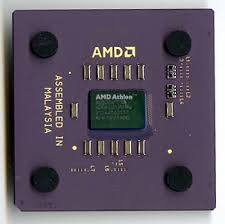
\includegraphics[width=0.2\textwidth]{figure/thunderbird.jpg}
    }
    \subfigure[Barton]{
        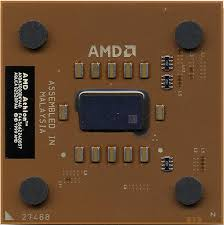
\includegraphics[width=0.2\textwidth]{figure/barton.jpg}
    }
    \caption{Athlon系列的后续产品}
\end{figure}

2001年,第四代Athlon(代号为Palomino)发布,定名为Athlon XP,将制程更新到了130nm。2003年,代号为Barton的第五代Athlon发布,集成了512KB的L2缓存,性能更上一层楼。而且,那时的发烧友正处于超频的黄金时代,而所有的Barton系列几乎均可超频至3GHz以上,满足了发烧友的要求。

\subsubsection{Duron系列:AMD的低端系列}

1998年,Intel在Pentium系列的基础上推出了Celeron系列处理器,作为应对,AMD也同样削弱了高端系列Athlon的L2缓存,推出了主打中低端的Duron(毒龙)系列。Duron系列一经推出,市场反响强烈。虽然L2缓存被砍了四分之三之多,然而Duron的缓存运行速度更快,更重要的是Duron的超频能力十分强大,再加上低廉的价格,成为了当时超频发烧友的不二之选。

关于Duron处理器,还有一个小故事:彼时的Duron系列由于超频能力过强,甚至在一定程度上影响了Athlon系列的销量,AMD不得已封锁了Duron的超频能力。然而不久,发烧友就找到了“锁频Duron”处理器的破解办法:将L1桥重新短接连通,就可以破解锁频。于是发烧友门尝试了锡焊、飞线、液金笔等连接方式均破解成功,最后甚至用铅笔画一道也能成功解锁,“铅笔破解法”从此流传开来,成了超频黄金时代里的一段佳话。
\begin{figure}[H]
    \begin{center}
        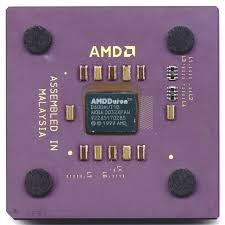
\includegraphics[width=0.2\textwidth]{figure/duron.jpg}
        \caption{AMD Duron处理器}
    \end{center}
\end{figure}

在随后的几年里,AMD的Athlon系列在高端产品线上持续与Intel Pentium系列抗衡,而没有推出Duron处理器来应对Celeron D,直到2003年新一代Duron(代号为Applebred)处理器发布。与初代Duron相同,AMD同样砍掉了Athlon系列部分L2缓存。然而,狂热的发烧友却不满足于此,他们又一次发现,Applebred只不过是屏蔽了Athlon系列上的部分L2缓存,玩家们通过短接L2桥,实现了“开核”,恢复成了完整的Athlon XP处理器!Duron系列的“开核”能力让它再一次成为了发烧友的绝佳选择。

\subsubsection{64位时代:Athlon产品线的再分布}

随着处理器的不断发展和对处理器寻址能力要求的不断提高,32位处理器已经不能满足需要。2001年,Intel推出了64位的Itanium(安腾)系列处理器,然而这一并不兼容x86架构的处理器并未成为主流,Intel也始终没有清晰的64位处理器计划。

然而,AMD又一次成功抓住了机会:2003年8月,AMD发布了新版的K8架构处理器,命名为Athlon 64。同时发布的还有Athlon 64 FX,又一次震惊世界。而且,这两款处理器与x86架构兼容,同时64位处理器也使得PC的内存不再局限于4GB,大大提高了CPU寻址的上限。时至今日,市面上主流的处理器均为64位处理器。
\begin{figure}[H]
    \centering
    \subfigure[AMD Athlon64]{
        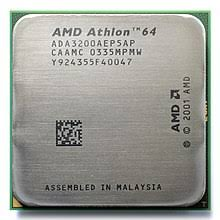
\includegraphics[width=0.2\textwidth]{figure/athlon64.jpg}
    }
    \subfigure[AMD Senpron系列徽标]{
        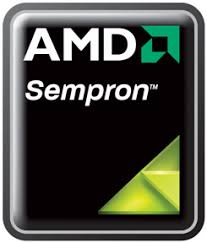
\includegraphics[width=0.17\textwidth]{figure/senpron.jpg}
    }
    \caption{AMD 64位时代的产品}
\end{figure}
Athlon 64系列处理器的L1和L2缓存分别高达128KB和1MB,主频最高达到了2.4GHz,晶体管数量也突破了1亿个,成为了当之无愧的“巨无霸”产品。同时他还向下兼容32位的x86架构,同时支持64位扩展,这使得原先为32位处理器编写的程序可以直接移植到Athlon 64上,大大提升了产品的适用性。Athlon 64系列在市场上也成功接过了Athlon XP系列的旗舰位置。

与此同时,AMD将其Athlon系列的产品线进行重新分配:Athlon 64系列主攻高端,Athlon 64 FX则为其中的旗舰产品;Duron系列与之前一样主攻中低端处理器;而原先的Athlon XP系列则被下放,以填补两者之间的空缺,同时AMD将其更名为Sempron(闪龙)系列。

\subsubsection{Athlon 64 X2:AMD这一时期的巅峰之作}
2005年,随着单核CPU的主频提升已经接近瓶颈,Intel和AMD不约而同地转向了多核心CPU的研发。费劲心思的Intel抢先发布了Pentium D系列双核处理器,AMD的Athlon 64 X2紧随其后。然而,Intel的双核方案只是将两个Pentium 4的总线相连,使用总线相互连接,又采用了Netburst架构,由此产生了巨额的发热和功耗,两个CPU核心的协同工作效果低下,因此被戏称为“胶水双核”。这一次的“真假双核”之争上,AMD以压倒性的优势获得了胜利。
\begin{figure}[H]
    \centering
    \subfigure[AMD Athlon 64 X2]{
        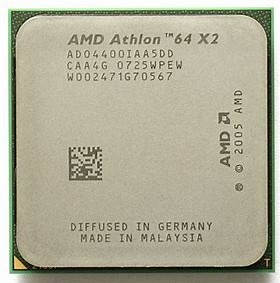
\includegraphics[width=0.2\textwidth]{figure/Athlon64X2.jpg}
    }
    \subfigure[“真假双核”之争]{
        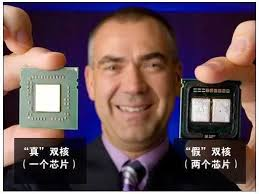
\includegraphics[width=0.27\textwidth]{figure/2core.jpg}
    }
    \caption{Athlon 64 X2与“真假双核”}
\end{figure}

初代的Athlon 64 X2处理器采用了90nm制程,后续又提升至65nm,提供了每个内核1MB的L2缓存,主频最高达到了2.4GHz。在同一块单晶硅上刻出了两个内核,无论是在两个核心的协同工作还是在发热的控制上都远超Pentium D系列。不夸张的说,Athlon 64 X2就是AMD Athlon系列的巅峰之作。

\subsection{2006-2017 AMD失落的十年}
2005年-2006年的AMD凭借这Athlon 64 X2的强势,在处理器市场上所向披靡。财大气粗的AMD于2006年7月收购了显卡巨头ATi,然而这是一把双刃剑。AMD在扩展了显卡业务的同时也陷入了资金流危机,在几年后不得不将其生产部门拆分成为GlobalFoundries Inc.(格罗方德公司)。同年,Intel Core 2 Duo系列的推出更是将AMD之前在CPU上的优势化为乌有。在内部和外部的双重打击下,AMD几近破产,进入了失落的十年。这一时期AMD新推出的产品有Phenon(羿龙)系列,Athlon2系列和FX系列。

\subsubsection{Phenon系列:失败的对抗产品}

2007年,为了应对Core系列的猛烈攻势,AMD推出了Phenon(羿龙)处理器予以应对。Phenon系列为四核处理器,除了每个核心独享的128KB一级缓存和512KB二级缓存外,还集成了共享的2MB三级缓存。由于架构上的差距,AMD在单核性能上完全无法与Intel的Core系列抗衡,只能堆起核心数。
\begin{figure}[H]
    \begin{center}
        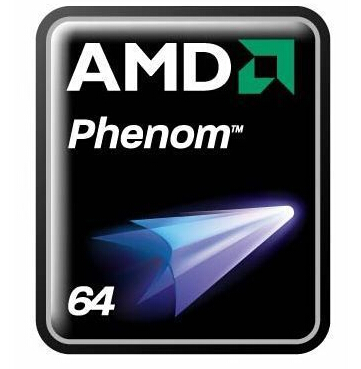
\includegraphics[width=0.2\textwidth]{figure/phenon.jpg}
        \caption{AMD Phenon系列徽标}
    \end{center}
\end{figure}
然而,被AMD寄予厚望的Phenon系列却在不久后遭遇了滑铁卢:在Phenon系列的B2步进核心出现了TLB错误,会导致CPU因自身错误而死机。这种bug无法通过软件层面弥补,只能更换CPU,AMD的声誉因而跌入谷底。

虽然2008年,AMD重新设计了适用于Phenon的B3步进核心,却仍然难以与同时期的Core 2竞争,只能退守中端市场。2009年,AMD的45nm制程Phenon\uppercase\expandafter{\romannumeral2}推出,然而同时期的Intel已经推出了i系列处理器。Phenon只能与最低端的i3竞争,面对i5和i7,AMD毫无办法,用Phenon对抗Core系列的策略也惨淡收场。

\subsubsection{Athlon2:令人唏嘘的下场}
2009年,AMD在中低端市场推出了Athlon2处理器,采用与Phenon\uppercase\expandafter{\romannumeral2}相同的K10架构,45nm制程,具有不错的超频能力,也因此在低端市场中占有一席之地,然而在高端产品上,AMD仍然无法与Intel抗衡。Athlon系列和Pentium系列一样,当初作为最新的高端产品推出,最后都被下放到低端产品线,令人唏嘘。

\subsubsection{FX系列:困境中艰难的赌注}

随着Phenon系列第一次对抗Core系列失败,AMD不得不进行新一轮的尝试。此时AMD想到了2006年收购的图形处理器生产商ATi,他们提出将图形处理器也集成在CPU中,即APU的构想。2011年,全新的Bulldozer(推土机)架构问世,该架构下的新款CPU被命名为AMD FX系列。

除了APU的设想以外,AMD还赌了一把,通过堆核心和高频长流水线来提升FX系列处理器的性能。然而,这样的赌注并没有取得成功,APU的设想兼容性太差,PC和游戏厂商适配热情不足,堆核心和高频长流水线的架构即使在32nm的制程下,仍然逃脱不了高功耗和发热的命运。
\begin{figure}[H]
    \begin{center}
        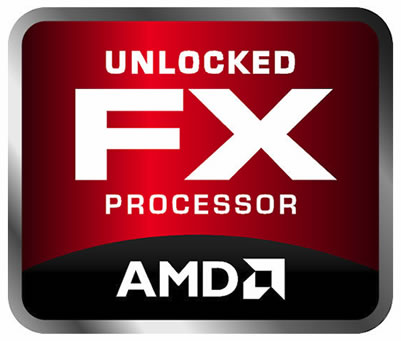
\includegraphics[width=0.2\textwidth]{figure/AMDFX.jpg}
        \caption{AMD FX系列徽标}
    \end{center}
\end{figure}
AMD FX系列日后还历经了Piledriver(打桩机),Steamroller(压路机),Excavator(挖掘机)三种同样以农机命名的微架构,AMD的戏称“农企”因此得名。但这些新的架构都是小修小补,没有真正的革命性变化,FX系列处理器始终反响平平,以至于竞争对手Intel开始对CPU性能“挤牙膏”等待AMD的步伐。


\subsection{2017-至今 锐龙(Ryzen)系列处理器与AMD的重生}
\subsubsection{初代Ryzen:转机的开始}
自2006年Intel推出了Core系列以来,AMD在十余年间都没有推出能与之相匹配的产品。然而事情的转机发生在2012年,当年研发K8架构的硬件架构师Jim Keller重回AMD,并宣布要重新设计底层架构,代号为Zen。

2017年,经过5年的等待,Zen架构处理器终于面世,AMD将其命名为Ryzen(锐龙)系列。Zen架构最大的变化在于紧追Intel在CPU中加入了超线程技术,且采用了模块化的设计,单个模块四核。模块化设计的好处是AMD可以通过堆叠相同的模块轻易达到超高的CPU核心数以提升性能,由此诞生了Threadripper(线程撕裂者)系列,初代Ryzen Threadripper最高达到了16核32线程。其次,模块下的每一个核心都独享一级缓存和二级缓存,只有三级缓存是单一模块下的核心共用,大大提高了核心的运行效率。在这一带CPU中,AMD放弃了APU的理念,集成了完整的整数核浮点计算单元,再加上14nm制程的运用,较好的控制了发热,Ryzen系列推出后,可以说AMD能够勉强追上了Intel的尾灯。
\begin{figure}[H]
    \begin{center}
        
\includegraphics[width=0.2\textwidth]{figure/ryzen.jpg}
        \caption{AMD Ryzen系列徽标}
    \end{center}
\end{figure}
Ryzen系列针对不同等级的消费者,从高到低分为Ryzen Threadripper,Ryzen 7,Ryzen 5,Ryzen 3系列处理器,涵盖了主流消费者的大部分需求。

\subsubsection{Ryzen系列的发展:AMD的重生}
一年后,AMD又发布了2代Ryzen处理器,架构为Zen架构改进而来的Zen+架构,采用12nm制程。与同时代的Intel在14nm挤牙膏相比,制程上的优势使得AMD在产品的竞争力上有了大的提升。2019年,采用7nm制程,采用第三代Zen2架构的Ryzen三代处理器发布。AMD在短短几年间完成了在技术指标上对Intel的超越。三代Ryzen在制程上的优势更加明显,AMD在之前一直为人所诟病的单核性能上,终于也能与Intel平起平坐了。此外,模块化的设计理念优势又一次体现:最高端的Ryzen Threadripper 3990X已经达到了令人夸张的64核128线程!
\begin{figure}[H]
    \begin{center}
        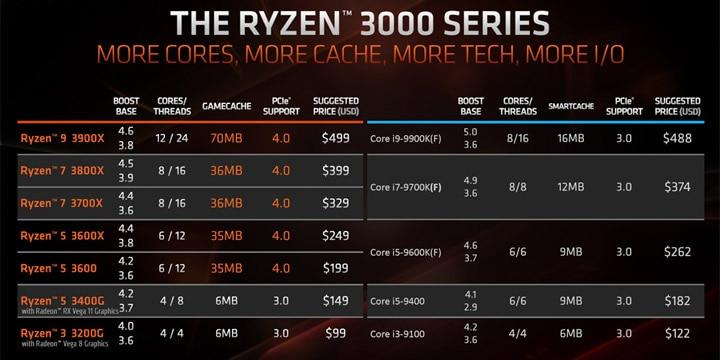
\includegraphics[width=0.6\textwidth]{figure/ryzen3.jpg}
        \caption{AMD Ryzen系列与Intel的对比}
    \end{center}
\end{figure}
2017年开始,这一股由Ryzen系列引发的AMD反扑浪潮,至今仍然在持续。从服务器、台式机到笔记本处理器,AMD在各个方面都追上甚至超过了Intel。AMD通过Ryzen系列成功浴火重生,一扫“农企”时期烂泥扶不上墙的形象。

\section{总结}

Intel与AMD,两家公司师出同源,而又在竞争激烈的CPU市场上角逐数十年。Intel在大部分时间主导着市场的发展,AMD则在大部分时间扮演“追赶者”,但偶尔也有高光时刻(比如现在)。两家公司角力的过程,也是微处理器一步步发展和完善的进程。CPU一直被称为人类工业品皇冠上的明珠,希望这两家公司能在未来让这颗明珠继续闪耀,也为我们奉献更多更精彩的故事。

\end{document}
